\section{Sri Rahayu (1174015)}
\subsection{Menulis Shapefile dengan PySHP}
\begin{enumerate}
	\item Nomor 1
	\lstinputlisting{src/1174015/2/No1.py}
	\begin{figure}[H]
		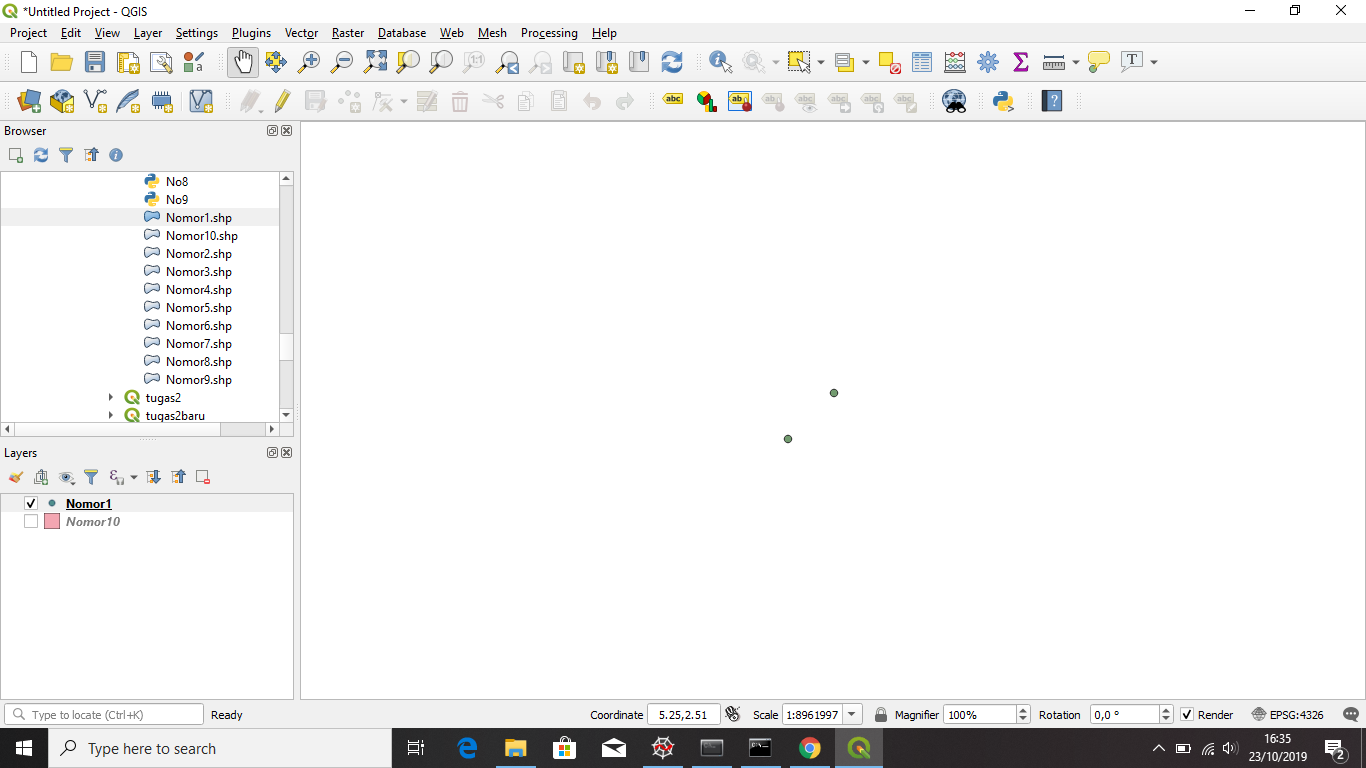
\includegraphics[width=6cm]{figures/1174015/2/No1.png}
		\centering
		\caption{Point (Titik)}
	\end{figure}
	\item Nomor 2
	\lstinputlisting{src/1174015/2/No2.py}
	\begin{figure}[H]
		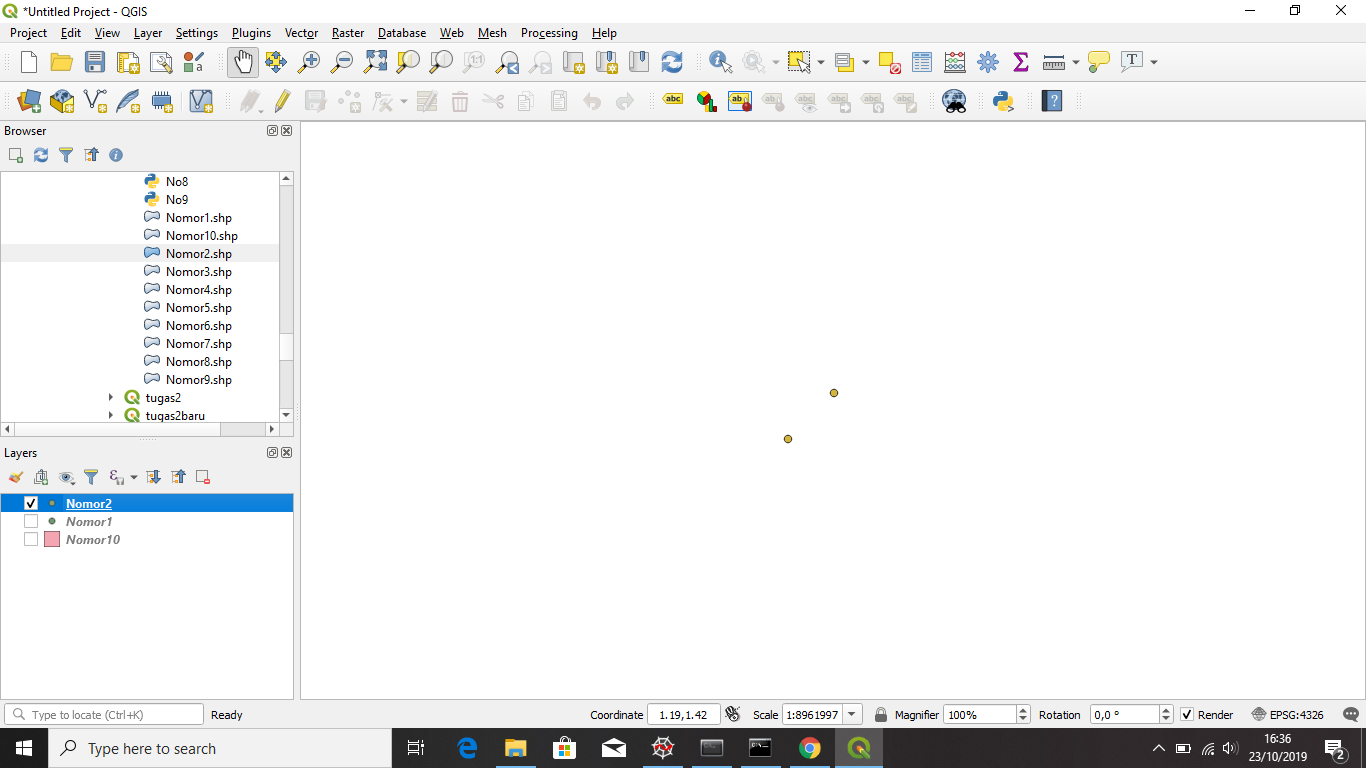
\includegraphics[width=6cm]{figures/1174015/2/No2.png}
		\centering
		\caption{Point (Titik)}
	\end{figure}
	\item Nomor 3
	\lstinputlisting{src/1174015/2/No3.py}
	\begin{figure}[H]
		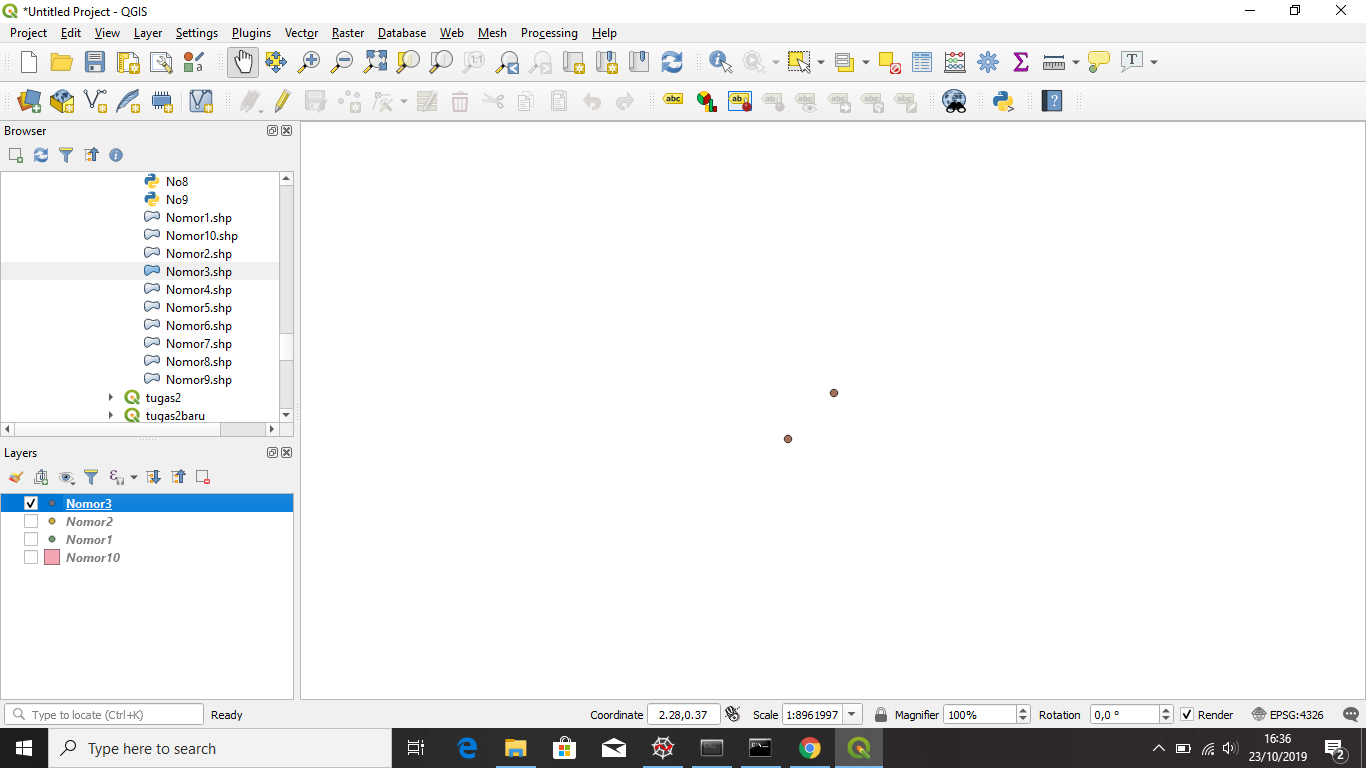
\includegraphics[width=6cm]{figures/1174015/2/No3.png}
		\centering
		\caption{Point (Titik)}
	\end{figure}
	\item Nomor 4
	\lstinputlisting{src/1174015/2/No4.py}
	\begin{figure}[H]
		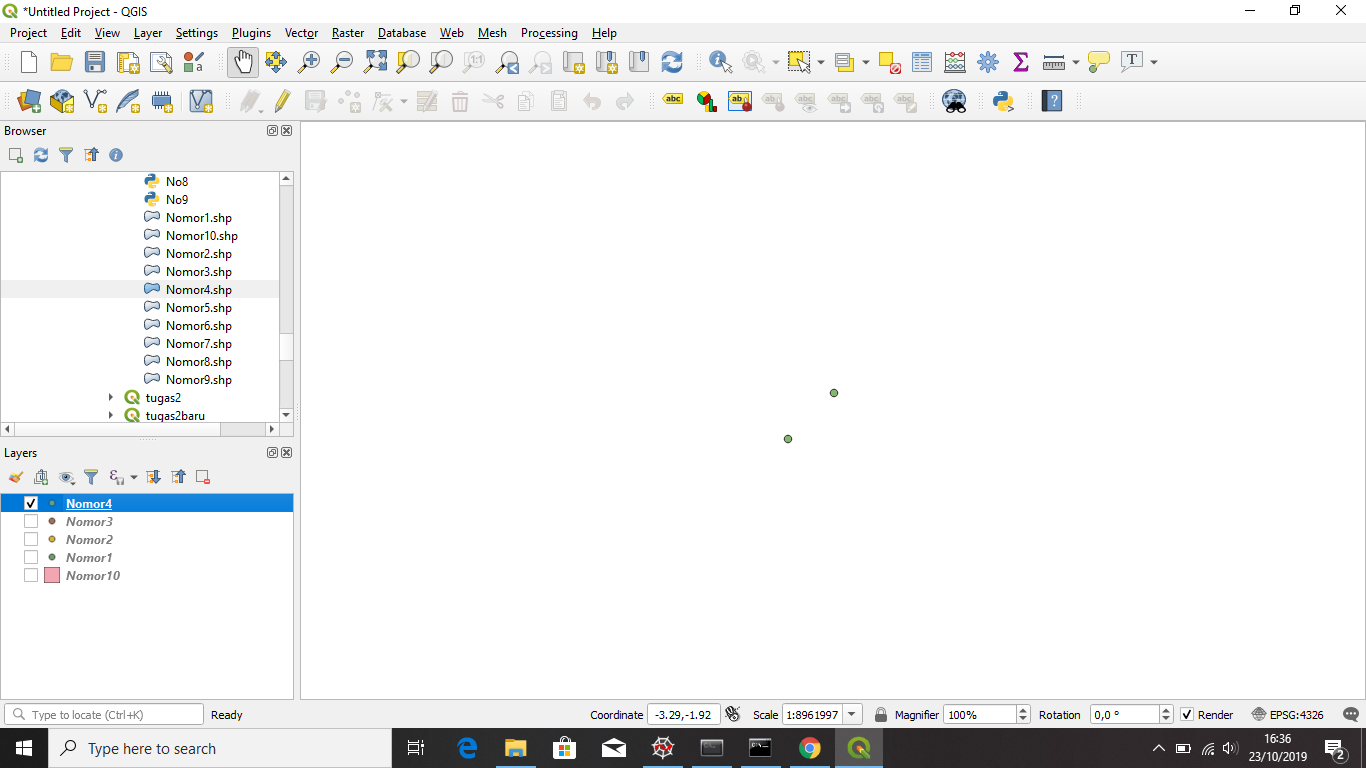
\includegraphics[width=6cm]{figures/1174015/2/No4.png}
		\centering
		\caption{Point (Titik)}
	\end{figure}
	\item Nomor 5
	\lstinputlisting{src/1174015/2/No5.py}
	\begin{figure}[H]
		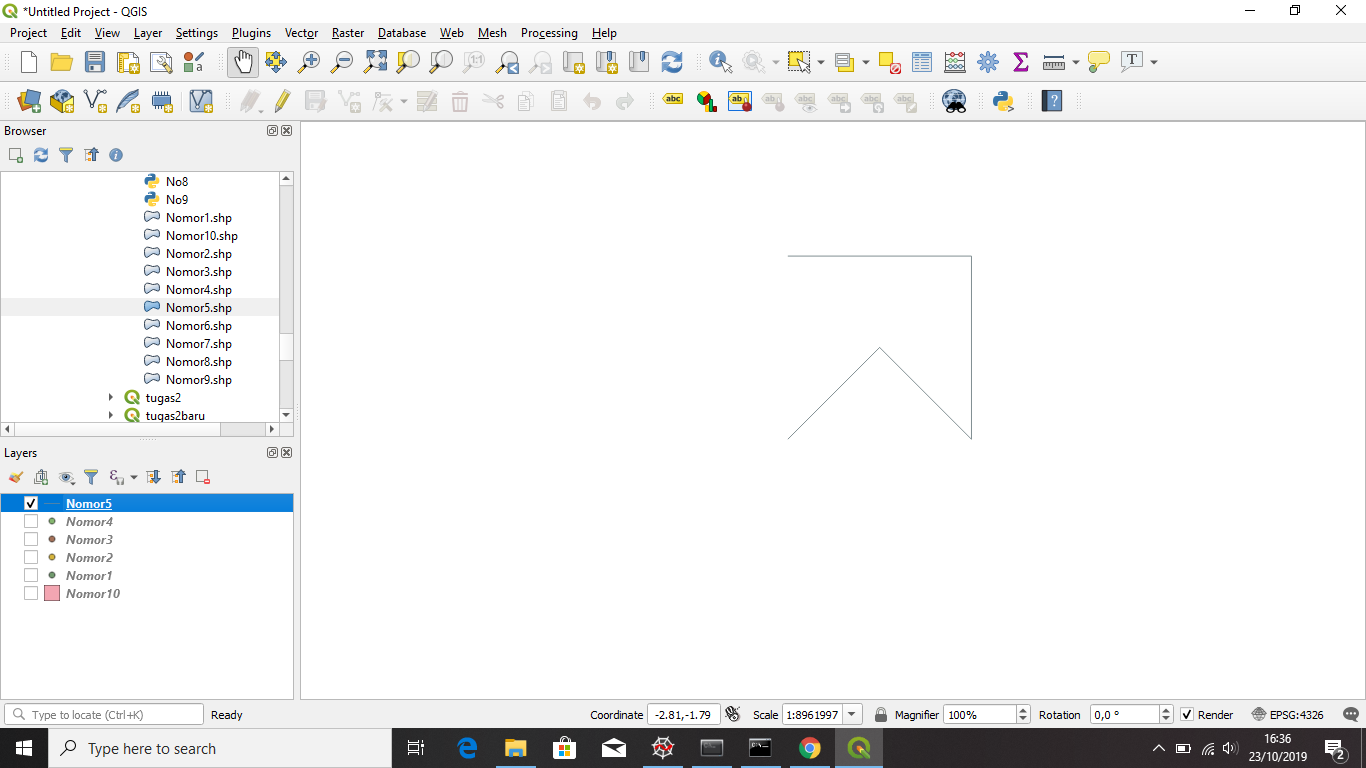
\includegraphics[width=6cm]{figures/1174015/2/No5.png}
		\centering
		\caption{PolyLine (Garis)}
	\end{figure}
	\item Nomor 6
	\lstinputlisting{src/1174015/2/No6.py}
	\begin{figure}[H]
		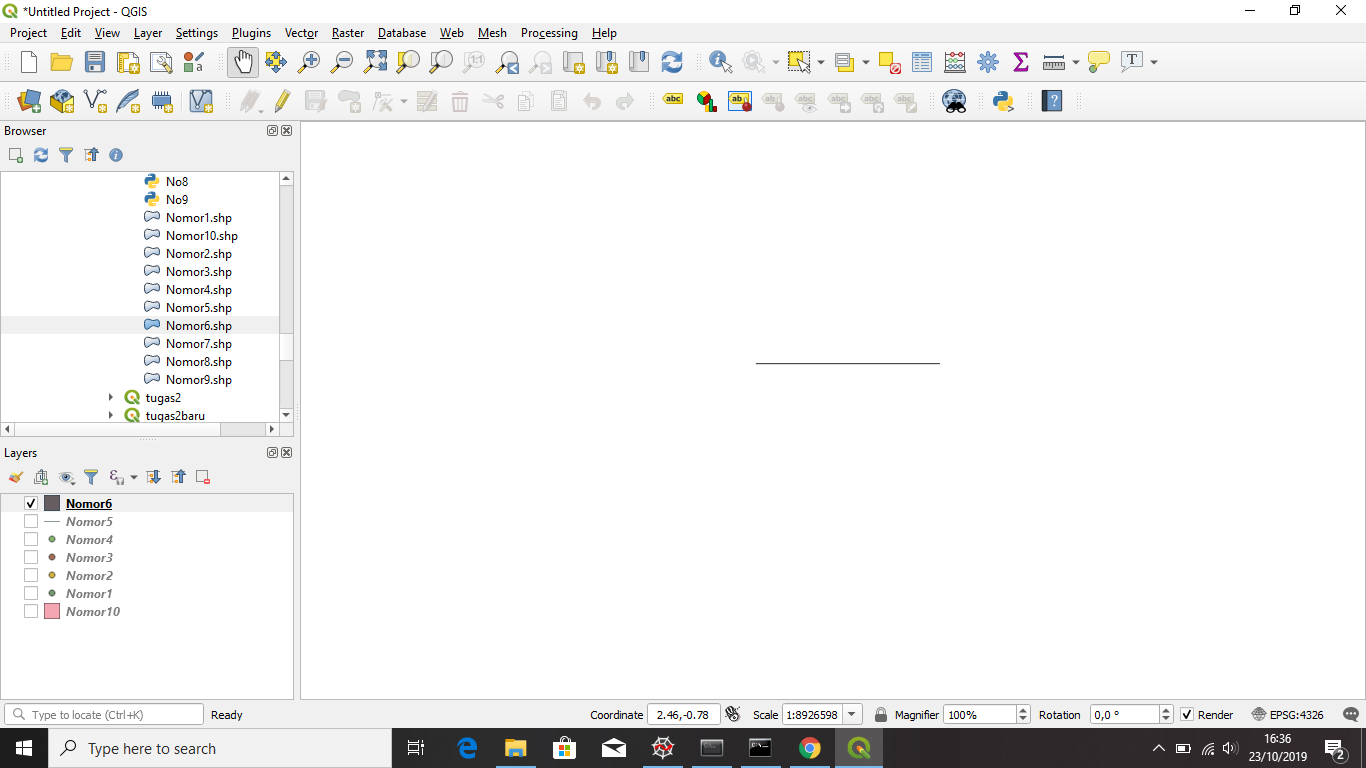
\includegraphics[width=6cm]{figures/1174015/2/No6.png}
		\centering
		\caption{Polygon (Bidang)}
	\end{figure}
	\item Nomor 7
	\lstinputlisting{src/1174015/2/No7.py}
	\begin{figure}[H]
		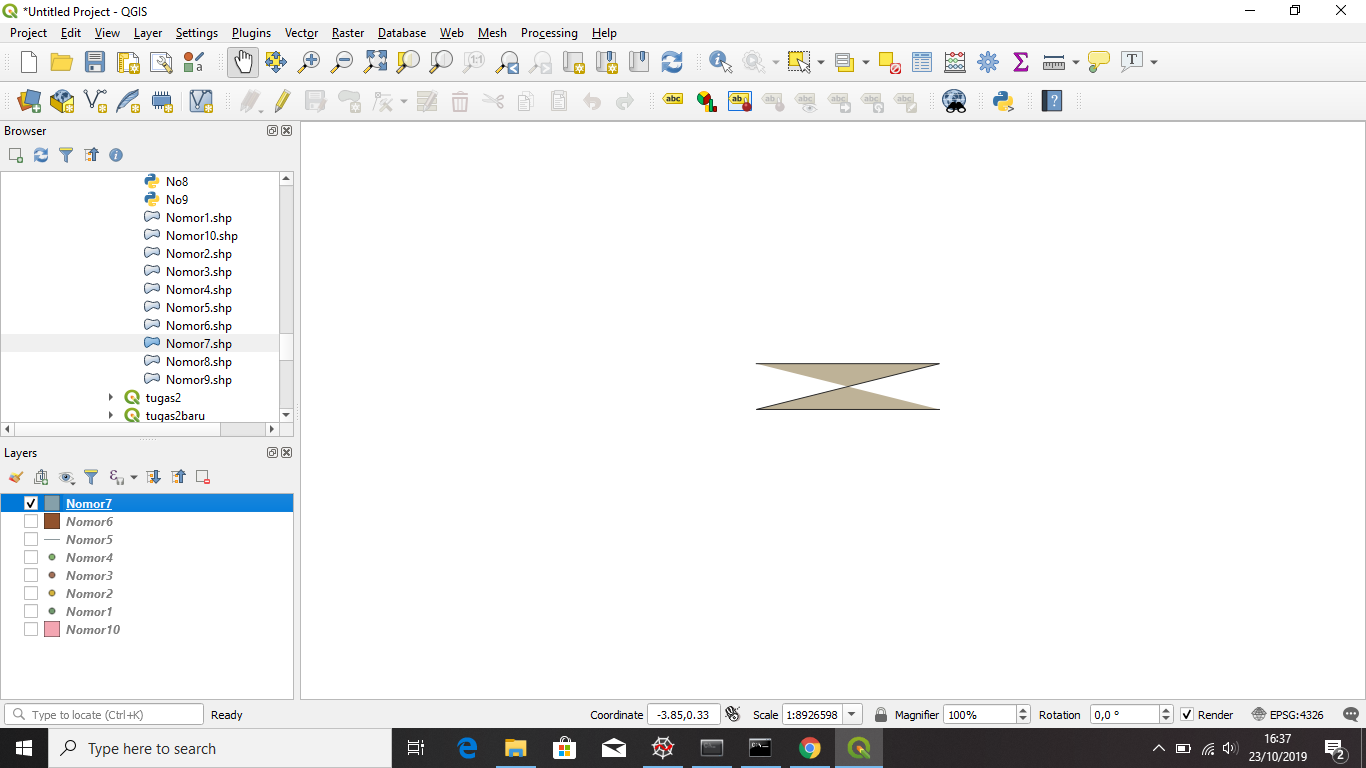
\includegraphics[width=6cm]{figures/1174015/2/No7.png}
		\centering
		\caption{Polygon (Bidang)}
	\end{figure}
	\item Nomor 8
	\lstinputlisting{src/1174015/2/No8.py}
	\begin{figure}[H]
		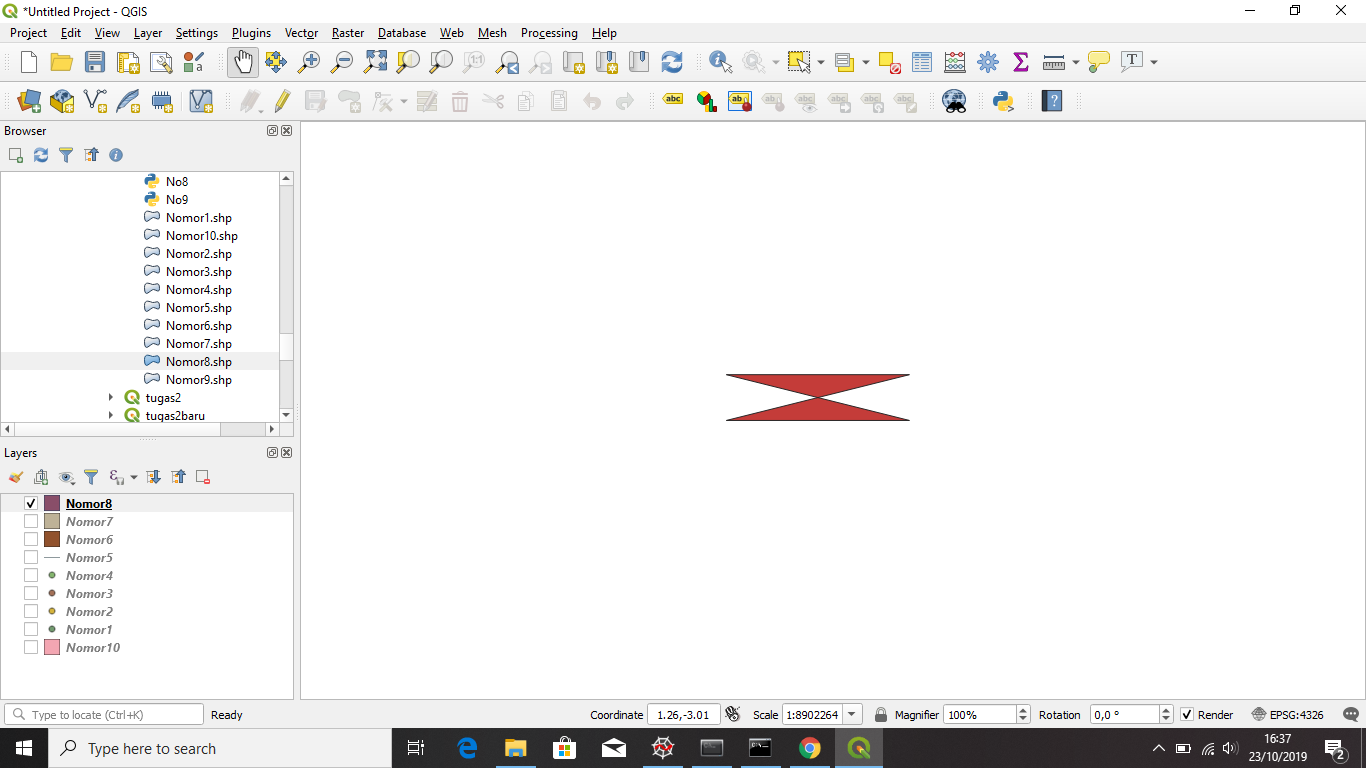
\includegraphics[width=6cm]{figures/1174015/2/No8.png}
		\centering
		\caption{Polygon (Bidang)}
	\end{figure}
	\item Nomor 9
	\lstinputlisting{src/1174015/2/No9.py}
	\begin{figure}[H]
		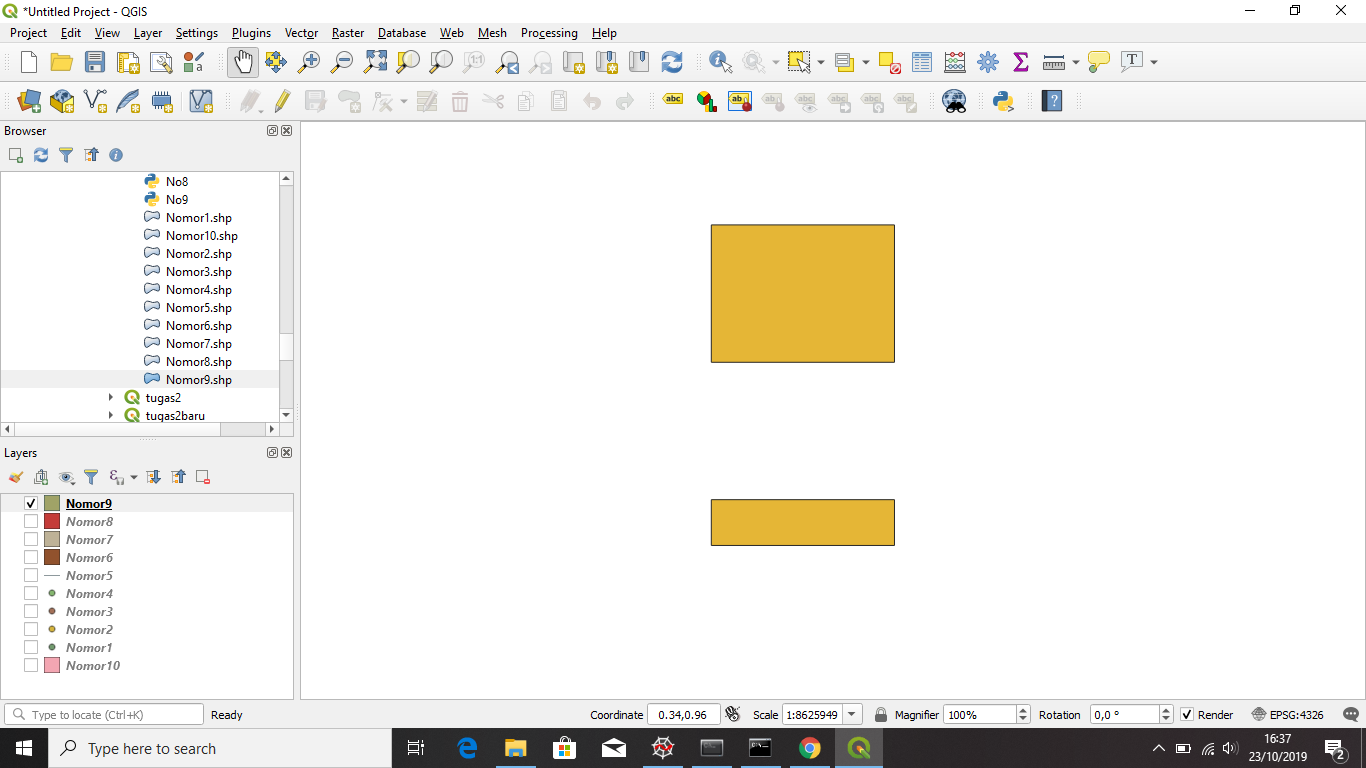
\includegraphics[width=6cm]{figures/1174015/2/No9.png}
		\centering
		\caption{Polygon (Bidang)}
	\end{figure}
	\item Nomor 10
	\lstinputlisting{src/1174015/2/No10.py}
	\begin{figure}[H]
		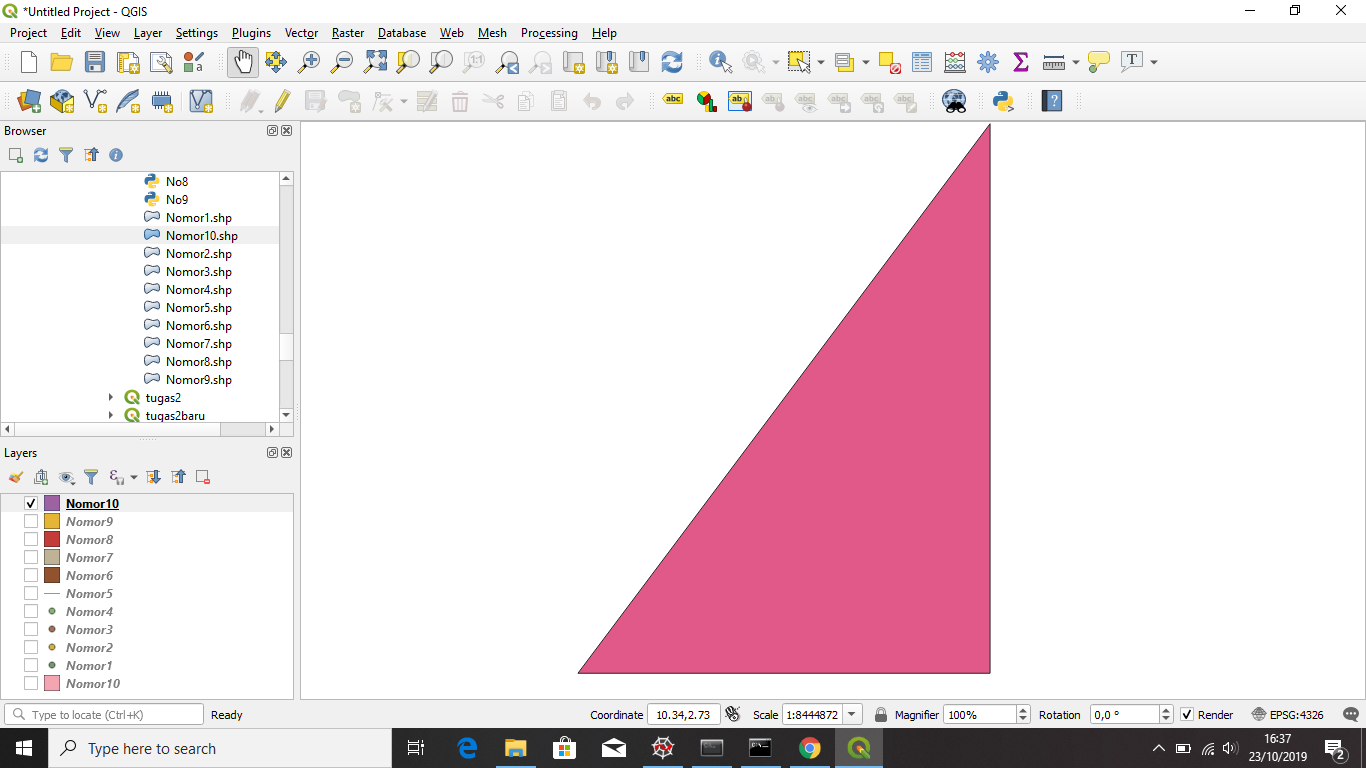
\includegraphics[width=6cm]{figures/1174015/2/No10.png}
		\centering
		\caption{Polygon,Hasil modul dari NPM saya 1174015 adalah 7 jadi membuat bidang siku siku sebanyak 1 buah }
	\end{figure}
\end{enumerate}
\subsection{Link}
https://youtu.be/MznvGwrD1kk